\section{Recombination Factor}

For the data-MC comparison, we use parameters of the recombination factor in ICARUS measurement of Ref.\cite{658352}.
In this section, we measure the recombination factor using proton (and Kaon) data.

% Electron-ion recombination depends on the electric field and stopping power $dE/dx$. We study this factor using tagged proton beam. 
%Recombination factor measurement using proton beam is relatively easy because of stability of proton. 
%This is why we used proton beam for this study as a first step.\\

  Expression for recombination (Birks law) in Eq.~\ref{eq:birkslaw} can can be rearranged like below:
\begin{equation}
  \frac{Q_{0}}{Q} = \frac{1}{A}+\frac{(k/E)(dE/dx)(1/\rho)}{A}
\end{equation}

In this equation, the ratio of $Q_{0}/Q$ has linear dependence of stopping power $dE/dx$,
and $Q$ from data (See Fig.~\ref{fig:Mean_comparison}), $Q_{0}$ and $dE/dx$ from MC can be determined for every distance from the stopped point.
By using this we are able to extract parameters $A$ and $k$.
$Q_{0}$ is determined from the simulation sample without recombination (Top left plot in Fig.~\ref{Fig:Preco}), and $dE/dx$ per an anode channel is determined with truth information of simulation (Top right plot in Fig.~\ref{Fig:Preco}). 
The result of this study is shown in bottom plot of Fig\ref{Fig:Preco}. Vertical axis is $Q_{0}/Q$, and horizontal axis is $dE/dx$ in this figure, this plot is fitted to straight line.
As a result, we obtain fitting parameter, $A$ = 0.832$\pm$0.009(stat.)$\pm$0.006(syst.), and $k$=0.0504$\pm$0.0010(stat.)$\pm$0.0013(syst.) [kV(g/cm$^{2}$)/cm/MeV]

It confirms Birks law in the range of 4  $\leqq$ dE/dx $\leqq$ 12 MeV/$cm^2$ and electric field of 200 V/cm is consistent with ICARUS measurement\cite{658352}.
 $A$ = 0.800$\pm$0.003 and $k$=0.0486$\pm$0.0006 [kV(g/cm$^{2}$)/cm/MeV]

%ch by ch data distribution
%\begin{figure}[!htb]
%  \begin{center}
%  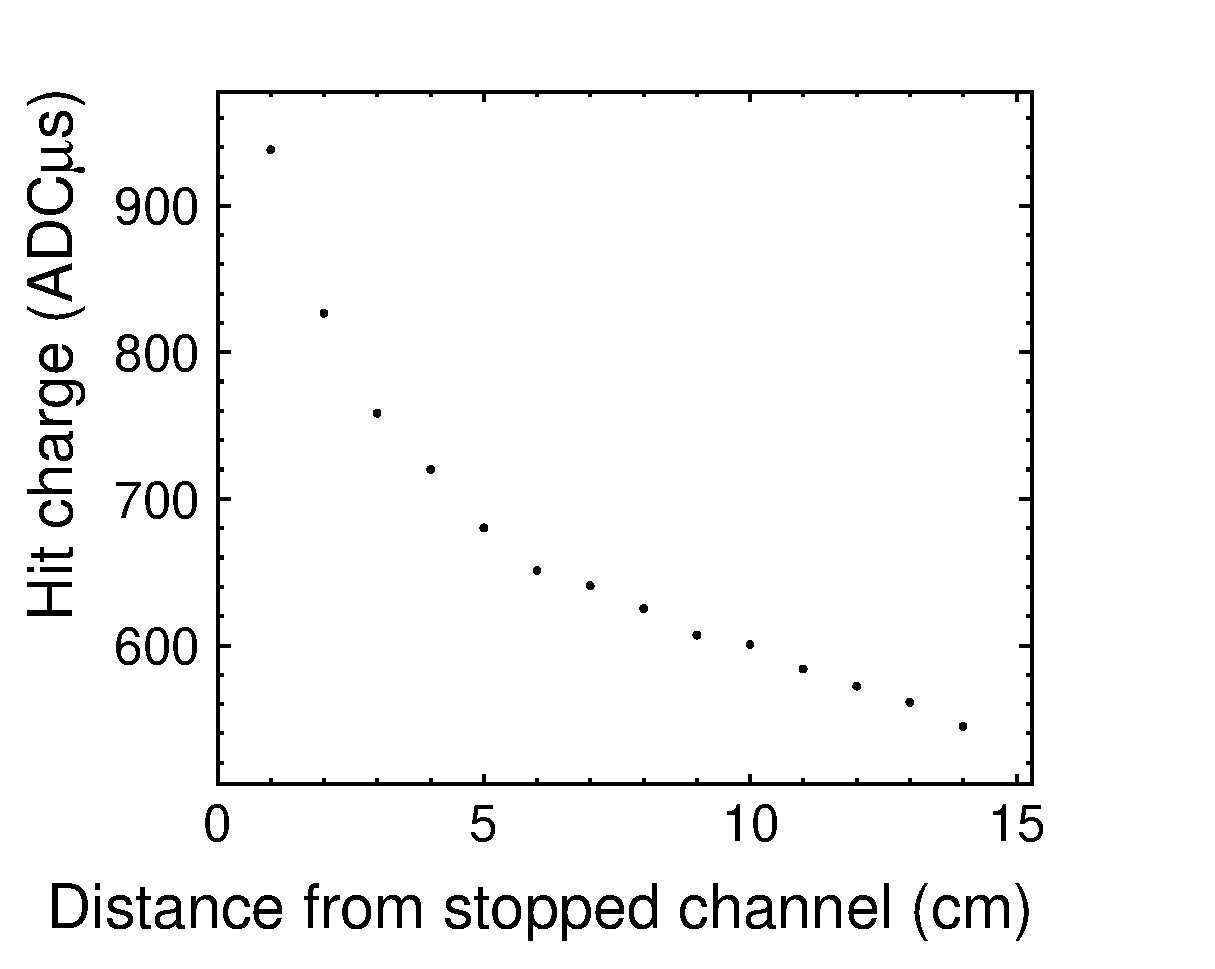
\includegraphics[0.3\hsize,clip]{./fig/Q2.eps}
%  \includegraphics[width=11cm,clip]{./fig/Data_FADCdistChbyCh.eps}
%  \caption{DATA:Integrated Flash ADC counts from stopped channel -1}
%  \label{fadcDist1}
%\end{figure}
%
%ch by ch MC distribution
\begin{figure}[!htb]
  \begin{center}
    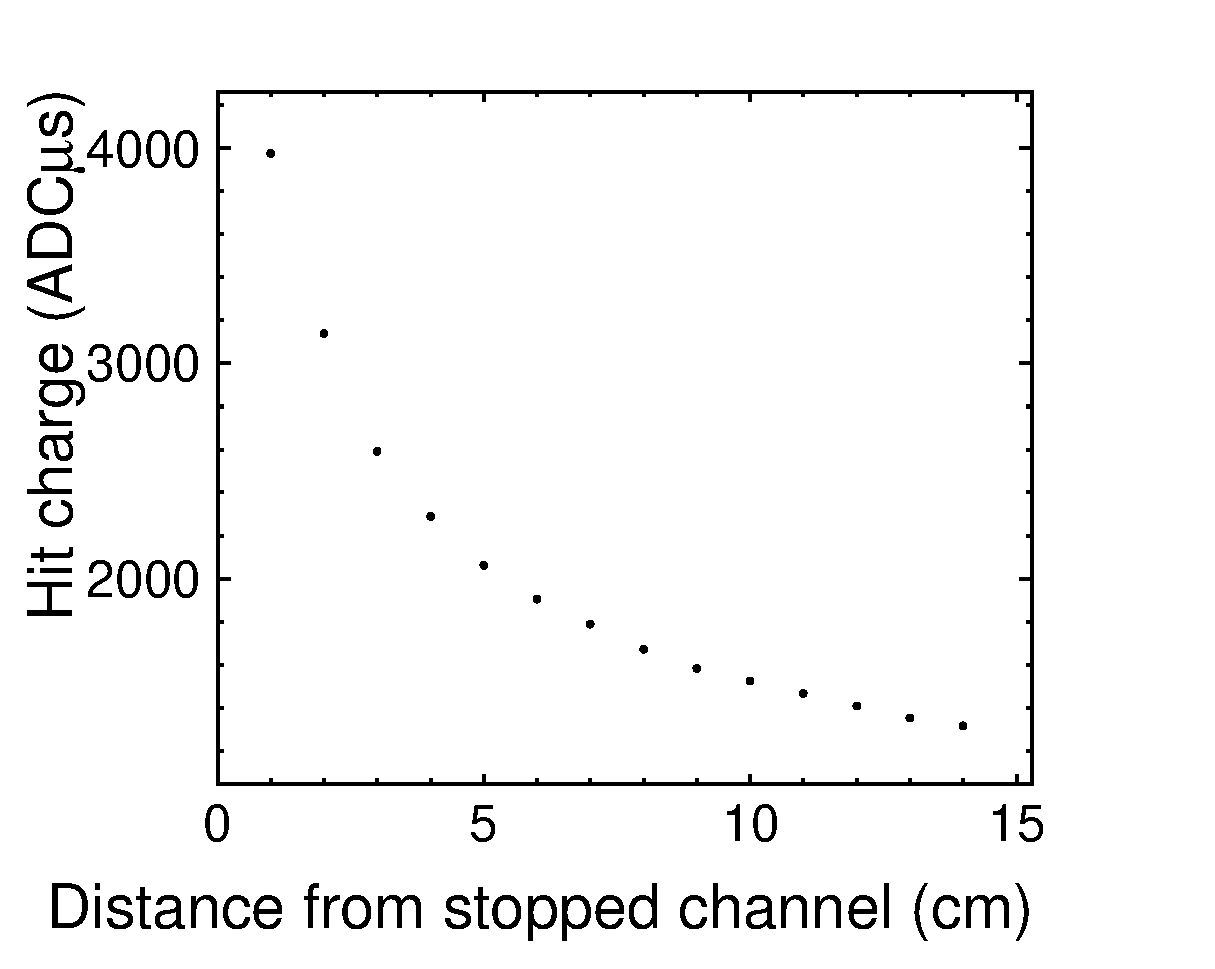
\includegraphics[width=0.45\hsize,clip]{./fig/Q_02.eps}
    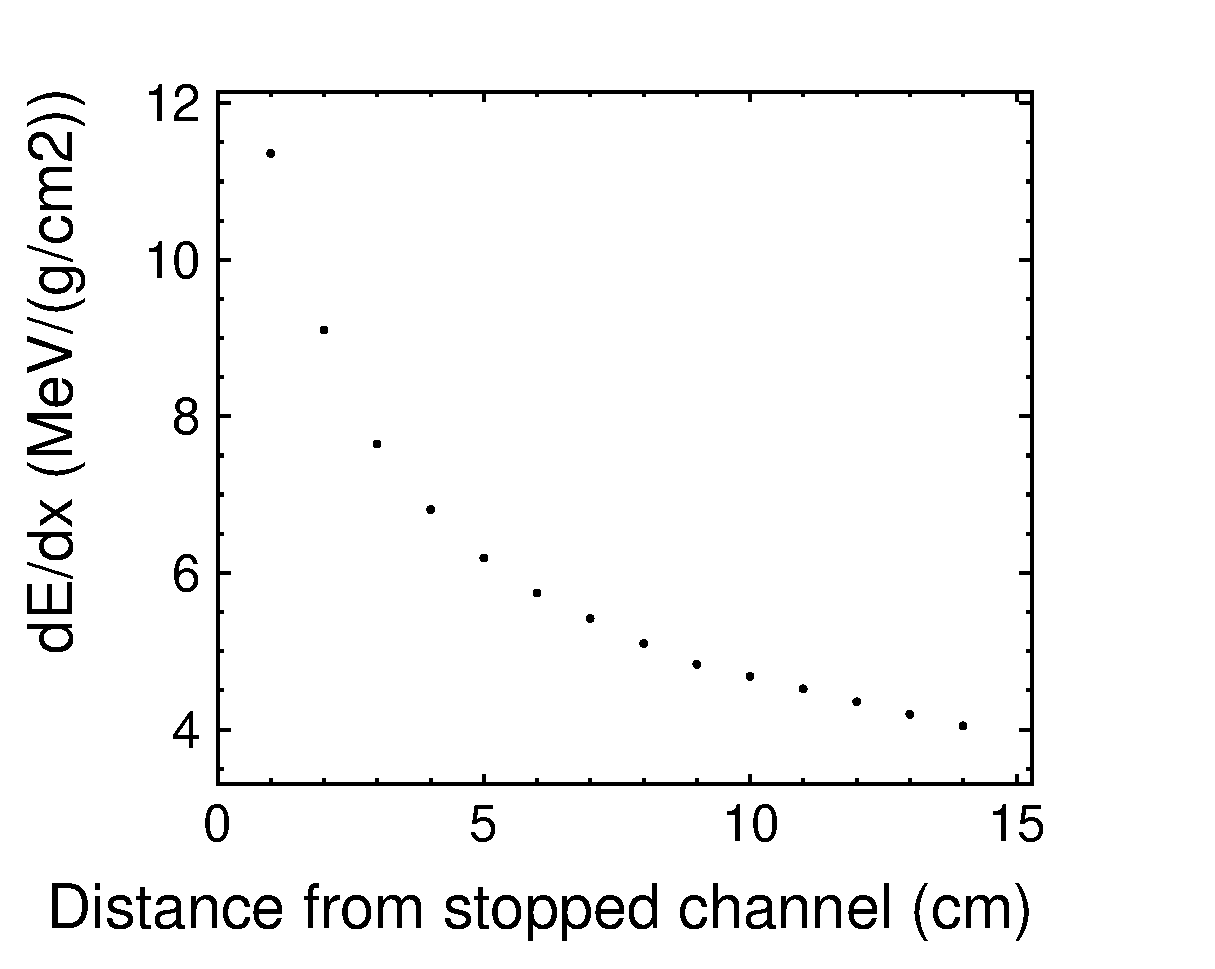
\includegraphics[width=0.45\hsize,clip]{./fig/dEdx2.eps}
    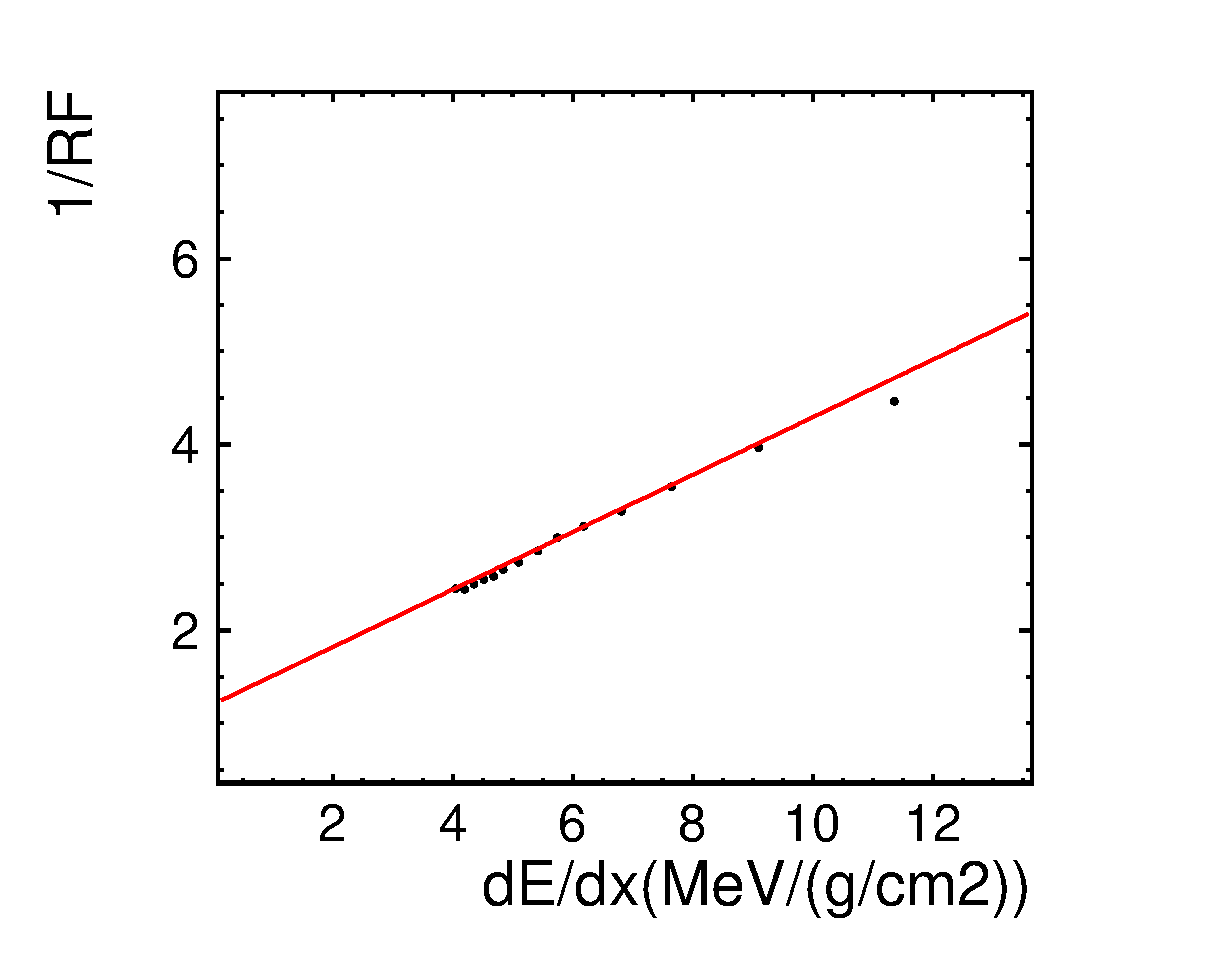
\includegraphics[width=0.8\hsize,clip]{./fig/RFresult2.eps}
    \caption{Top left and top right plots show simulated hit charge without recombination ($Q_0$) and
      average energy deposition ($dE/dx$) respectively as a function of the distance from the proton stopped point,
      and bottom plot shows 1/RF VS dE/dx fitted by Birks law}
    %  \caption{Distribution of dE/dx ch by ch}
    %  \caption{dE/dx from stopped channel -1}
    \label{Fig:Preco}
  \end{center}
\end{figure}
%
%result

%\begin{figure}[!htb]
%  \centering
%  \centering
%  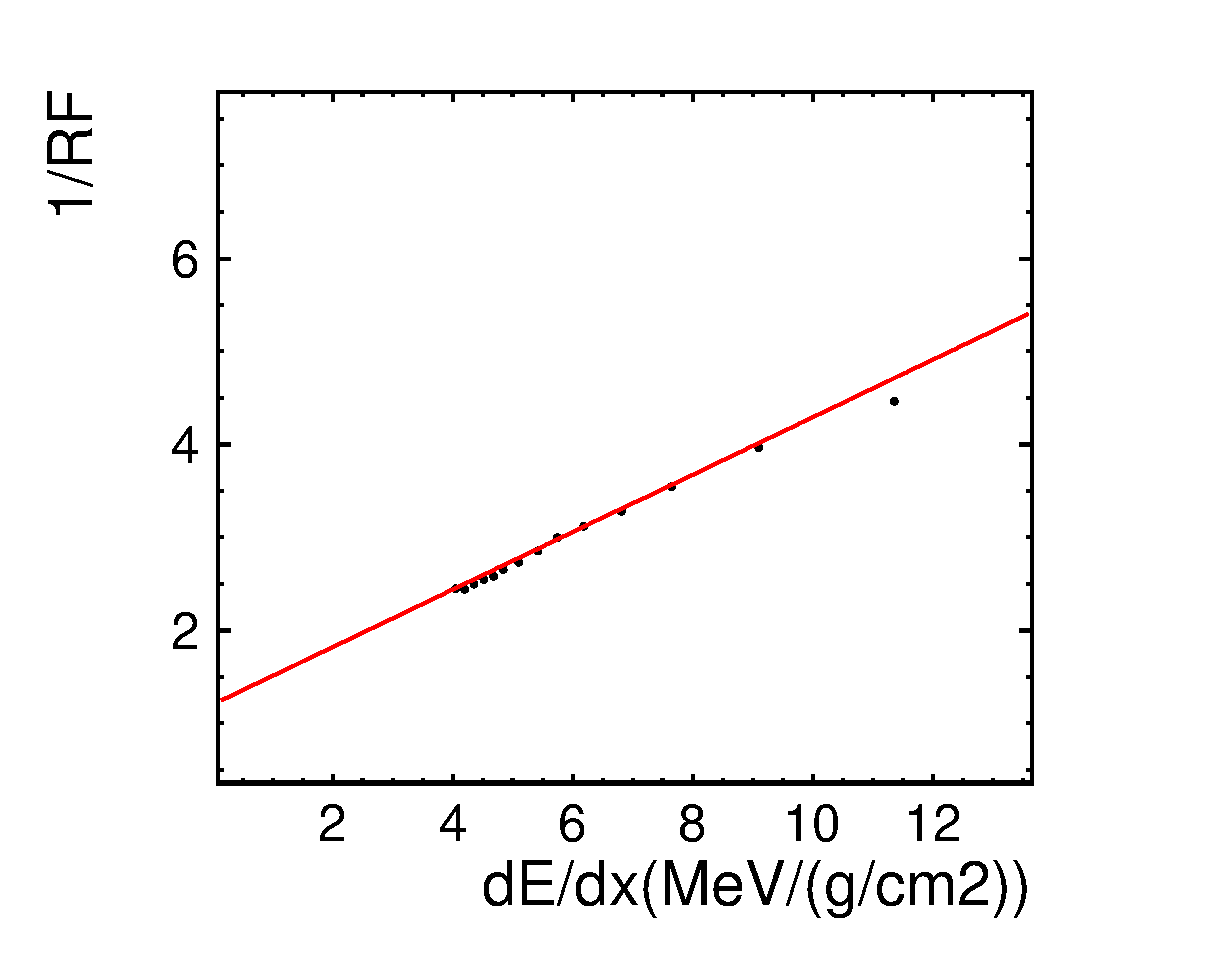
\includegraphics[width=0.8\hsize,clip]{./fig/RFresult2.eps}
%  \caption{1/RF VS dE/dx: fitted by Birks law}
%  \label{result}
%\end{figure}
